\documentclass[10pt,utf8]{beamer}

\mode<presentation> {
  \usetheme{Madrid}
  \setbeamercovered{transparent}
}

\usepackage{palatino}
\usepackage{graphicx}
\usepackage{array}
\usepackage{color}
\usepackage{subfigure}
\usepackage{colortbl}
\usepackage{amsmath}
\usepackage{hyperref}
\usepackage{listings}
\usepackage{pythonhighlight} % dnf install texlive-pythonhighlight
\usepackage{lmodern}

\setbeamertemplate{caption}{\raggedright\insertcaption\par} %turn off caption prefix ("Figure")

\definecolor{delim}{RGB}{20,105,176}
\definecolor{numb}{RGB}{106, 109, 32}
\definecolor{string}{rgb}{0.64,0.08,0.08}

% Define JSON language style
% Taken from https://gist.github.com/ed-cooper/1927af4ccac39b083440d436d018d253
\lstdefinelanguage{json}{
    showspaces=false,
    showtabs=false,
    breaklines=true,
    %postbreak=\raisebox{0ex}[0ex][0ex]{\ensuremath{\color{gray}\hookrightarrow\space}},
    breakatwhitespace=true,
    basicstyle=\ttfamily\footnotesize,
    upquote=true,
    morestring=[b]",
    stringstyle=\color{string},
    literate=
     *{0}{{{\color{numb}0}}}{1}
      {1}{{{\color{numb}1}}}{1}
      {2}{{{\color{numb}2}}}{1}
      {3}{{{\color{numb}3}}}{1}
      {4}{{{\color{numb}4}}}{1}
      {5}{{{\color{numb}5}}}{1}
      {6}{{{\color{numb}6}}}{1}
      {7}{{{\color{numb}7}}}{1}
      {8}{{{\color{numb}8}}}{1}
      {9}{{{\color{numb}9}}}{1}
      {\{}{{{\color{delim}{\{}}}}{1}
      {\}}{{{\color{delim}{\}}}}}{1}
      {[}{{{\color{delim}{[}}}}{1}
      {]}{{{\color{delim}{]}}}}{1},
}


\title{Feeding ML models with the data from the databases in real-time }
\author{Vojtěch Juránek}
\institute[Red Hat]{Red Hat}
\date{June 15th 2024, DevConf, Brno}

\newenvironment{mylisting}
{\begin{list}{}{\setlength{\leftmargin}{1em}}\item\scriptsize\bfseries}
{\end{list}}

\newenvironment{mytinylisting}
{\begin{list}{}{\setlength{\leftmargin}{1em}}\item\tiny\bfseries}
{\end{list}}


\begin{document}

%\tikzstyle{every picture}+=[remember picture]
%\tikzstyle{na} = [baseline=-.5ex]

\begin{frame}
    \centering
    \huge{\textbf{Let's start with the demo!}}
    \vspace{1cm}
    \begin{figure}
        \centering
        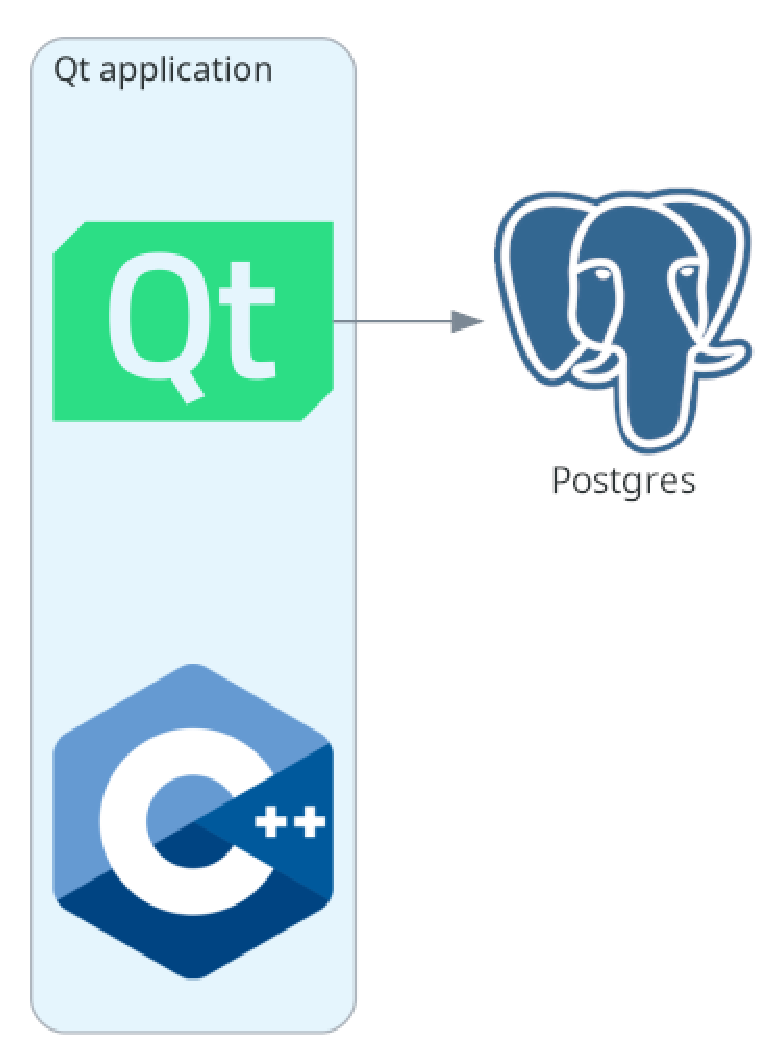
\includegraphics[height=5cm]{./img/qt_to_postgres.eps}
    \end{figure}
\end{frame}

\begin{frame}
 \titlepage
\end{frame}


\begin{frame}
    \begin{figure}
        \centering
        \includegraphics[height=8cm]{./img/mlops.eps}
        \caption{\tiny{Source: \url{https://ml-ops.org/content/end-to-end-ml-workflow}}}
    \end{figure}
\end{frame}

\begin{frame}
    \begin{figure}
        \centering
        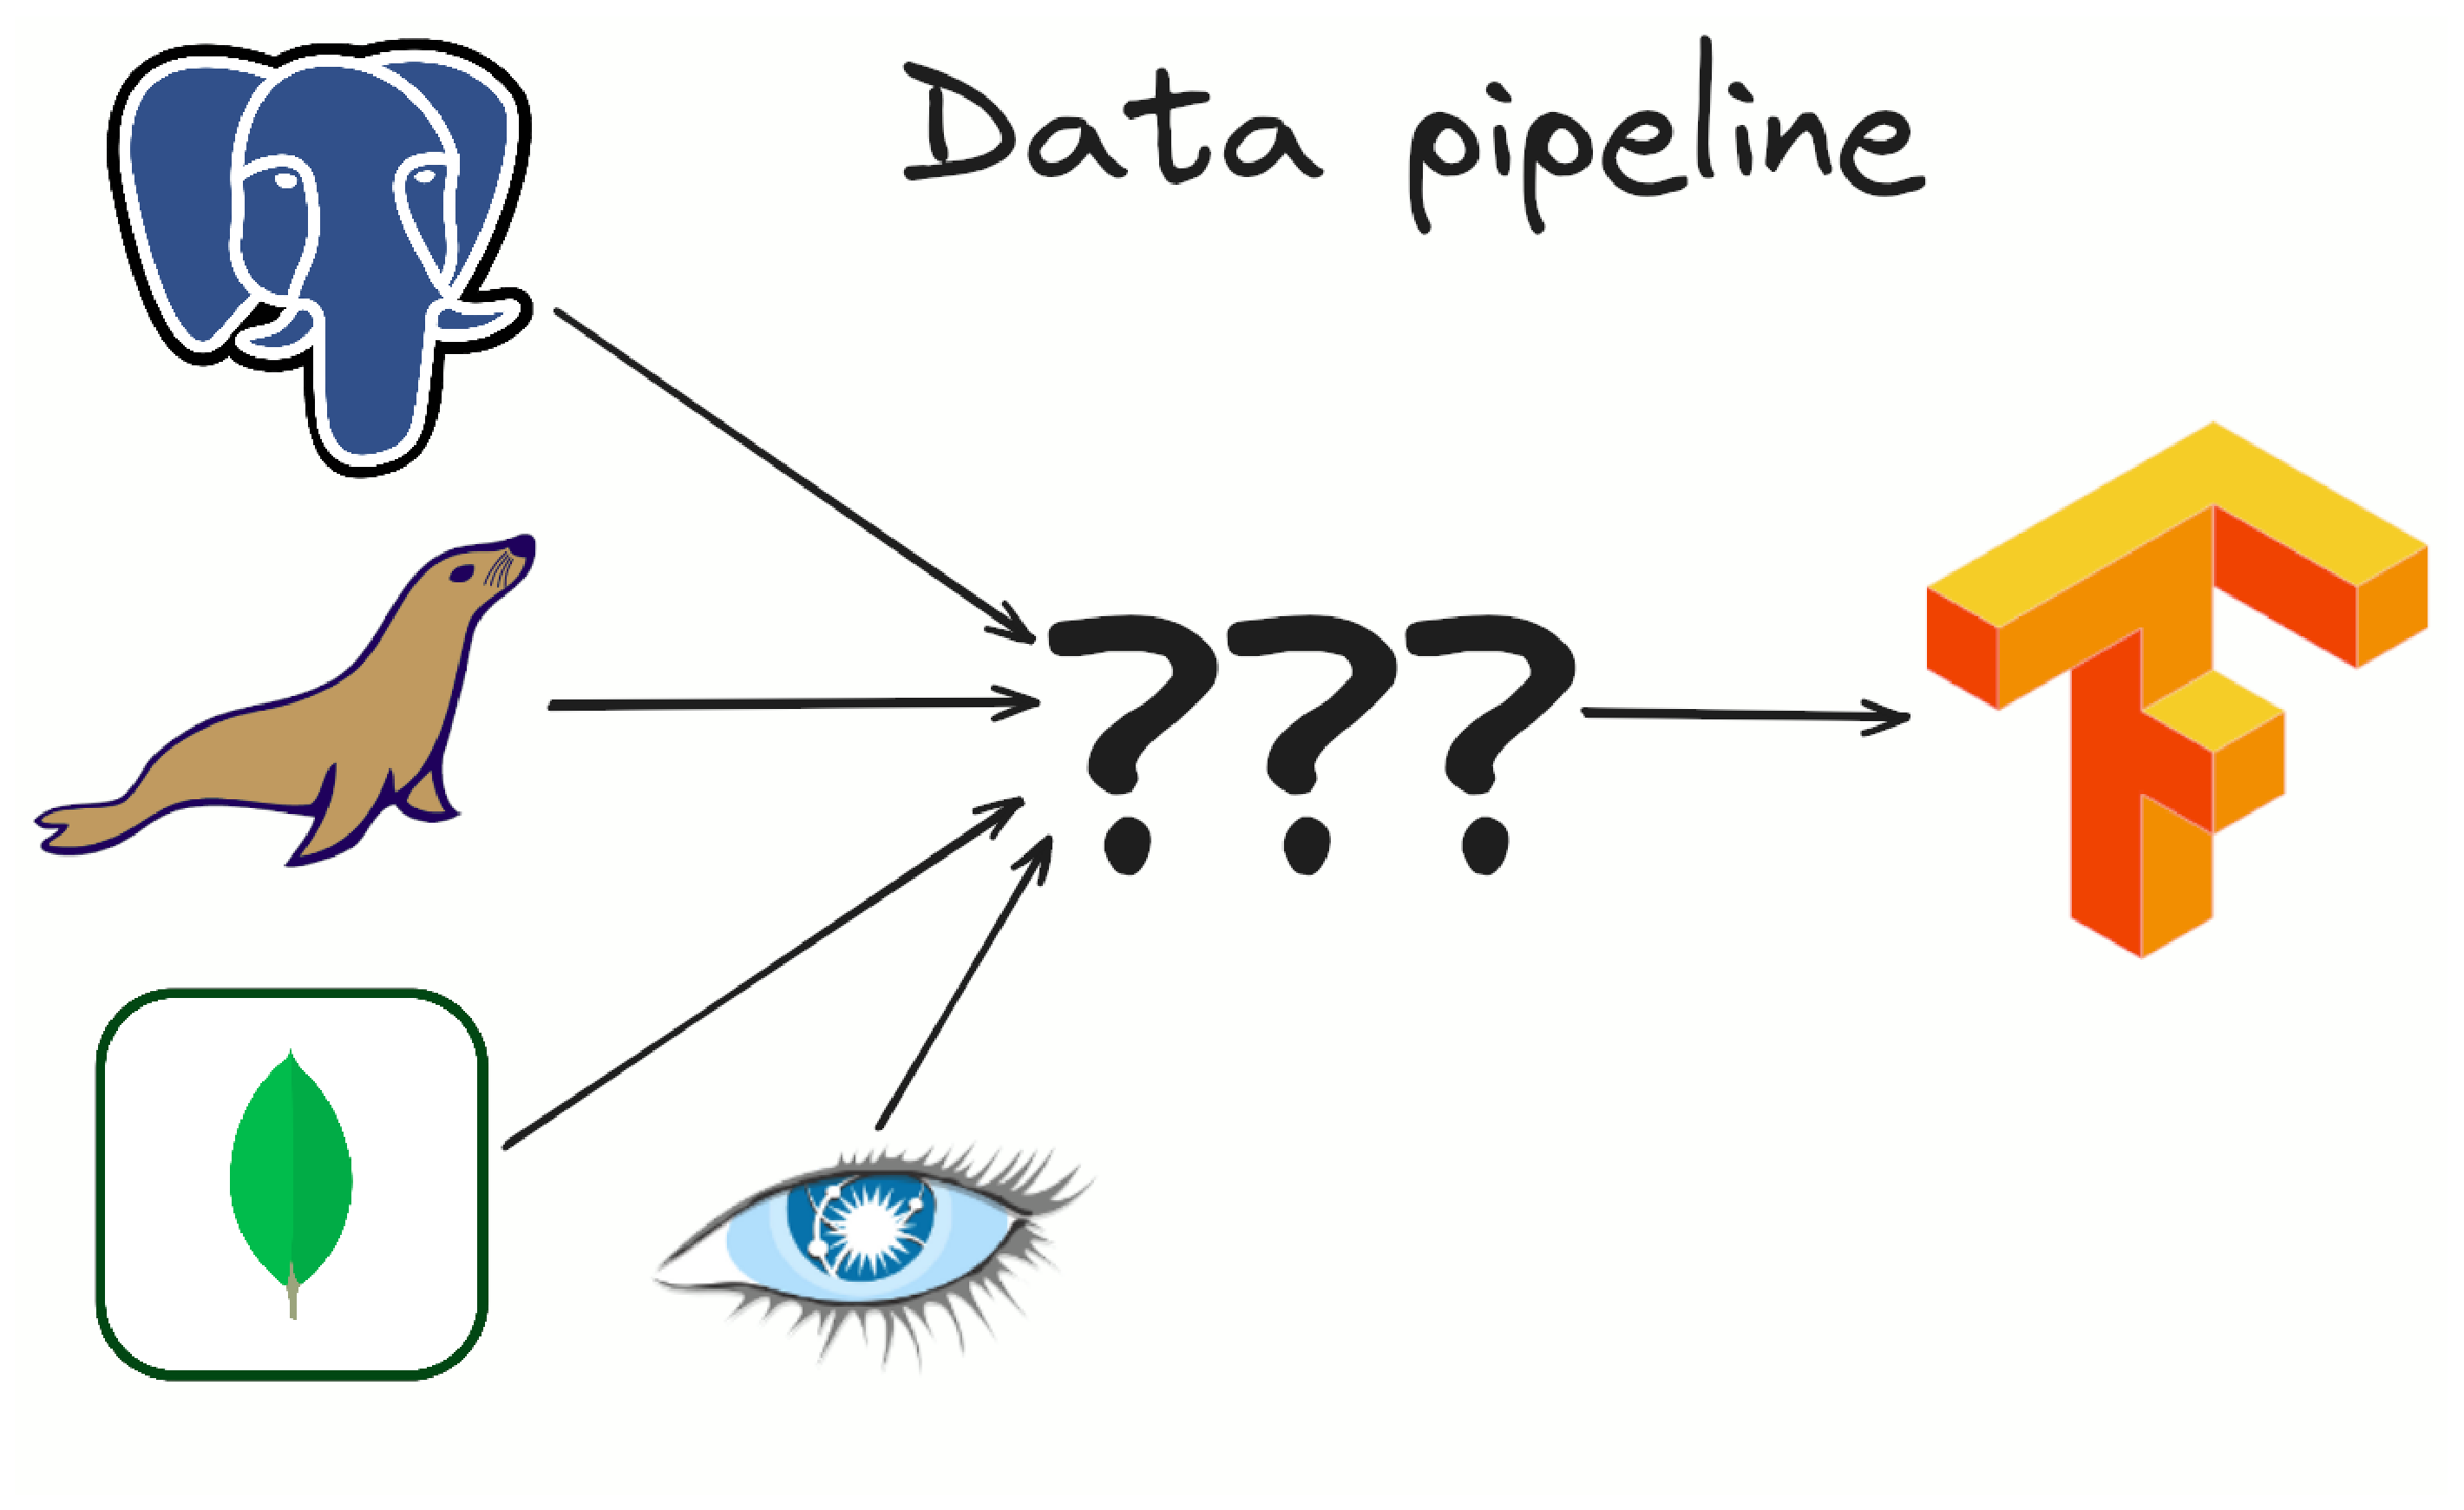
\includegraphics[height=7cm]{./img/dbs_to_tf2.eps}
    \end{figure}
\end{frame}

\begin{frame}
    \begin{figure}
        \centering
        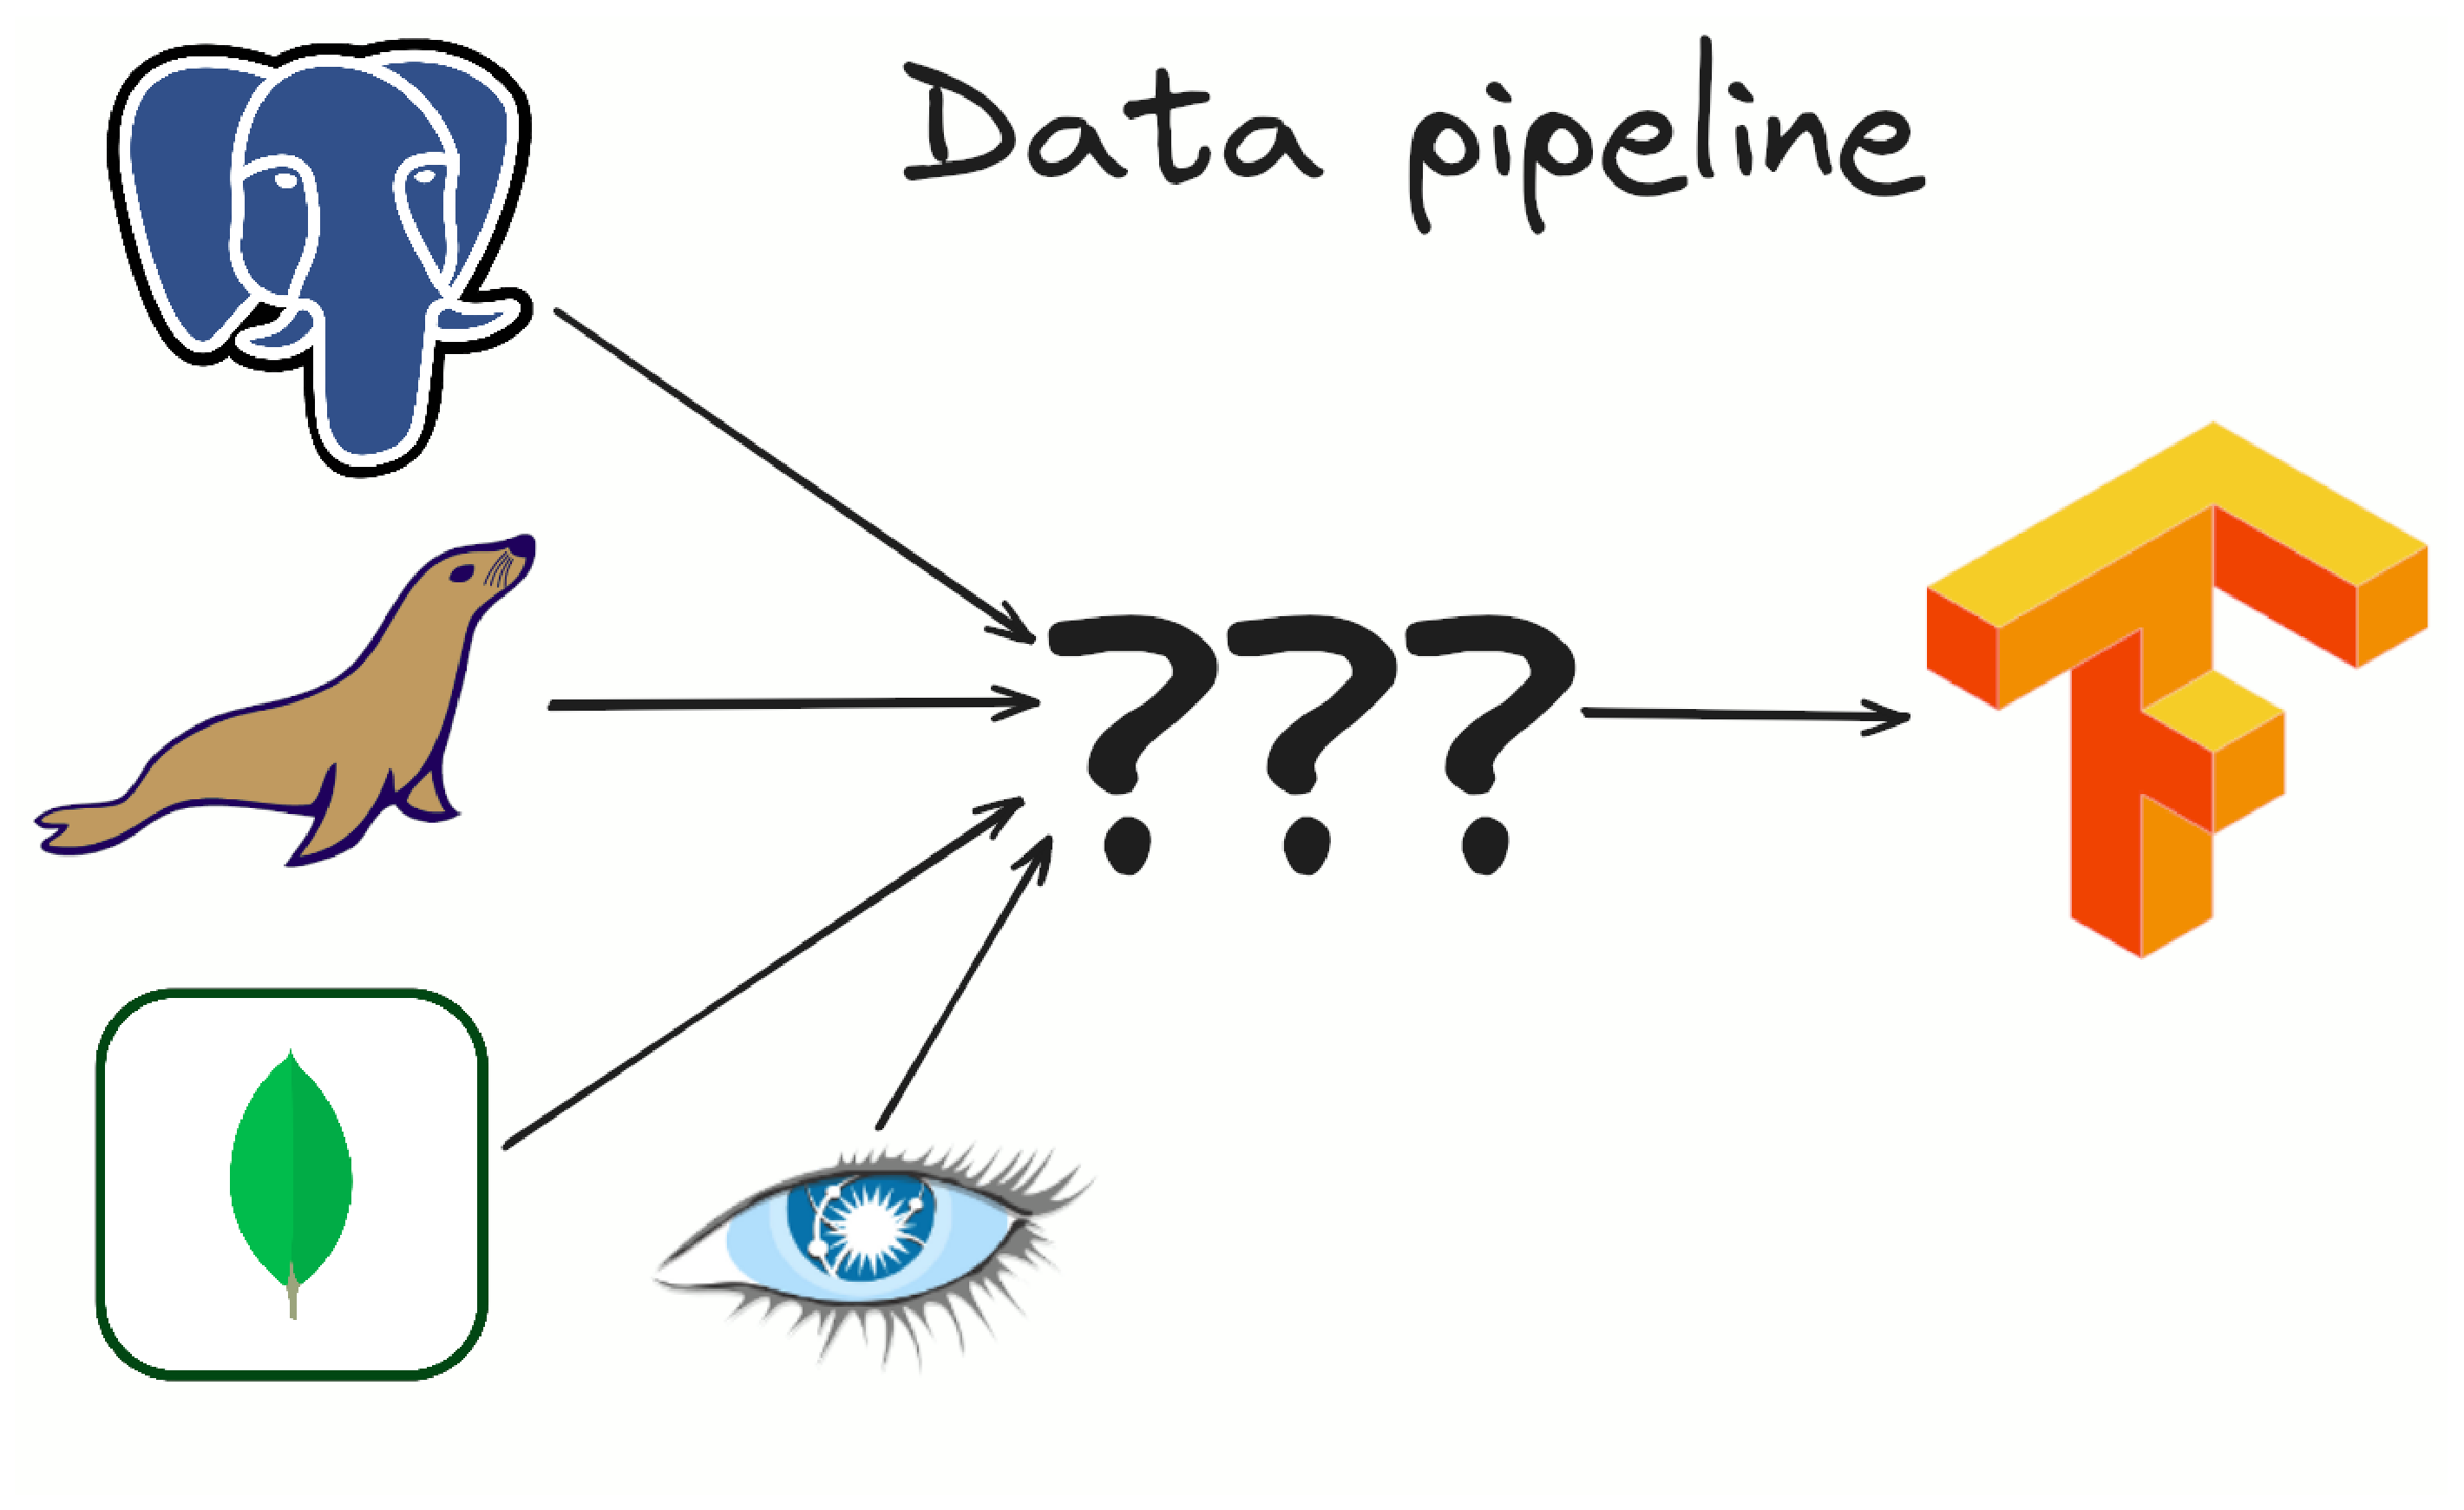
\includegraphics[height=3cm]{./img/dbs_to_tf2.eps}
    \end{figure}
    \begin{itemize}
      \item Consistent data, no data losses, no dual writes.
      \item Get all the changes without any delay in the real-time.
      \item Not overload the DB with the queries.
    \end{itemize}
\end{frame}

\begin{frame}
   % \frametitle{Change Data Capture (CDC)}
    \begin{figure}
        \centering
        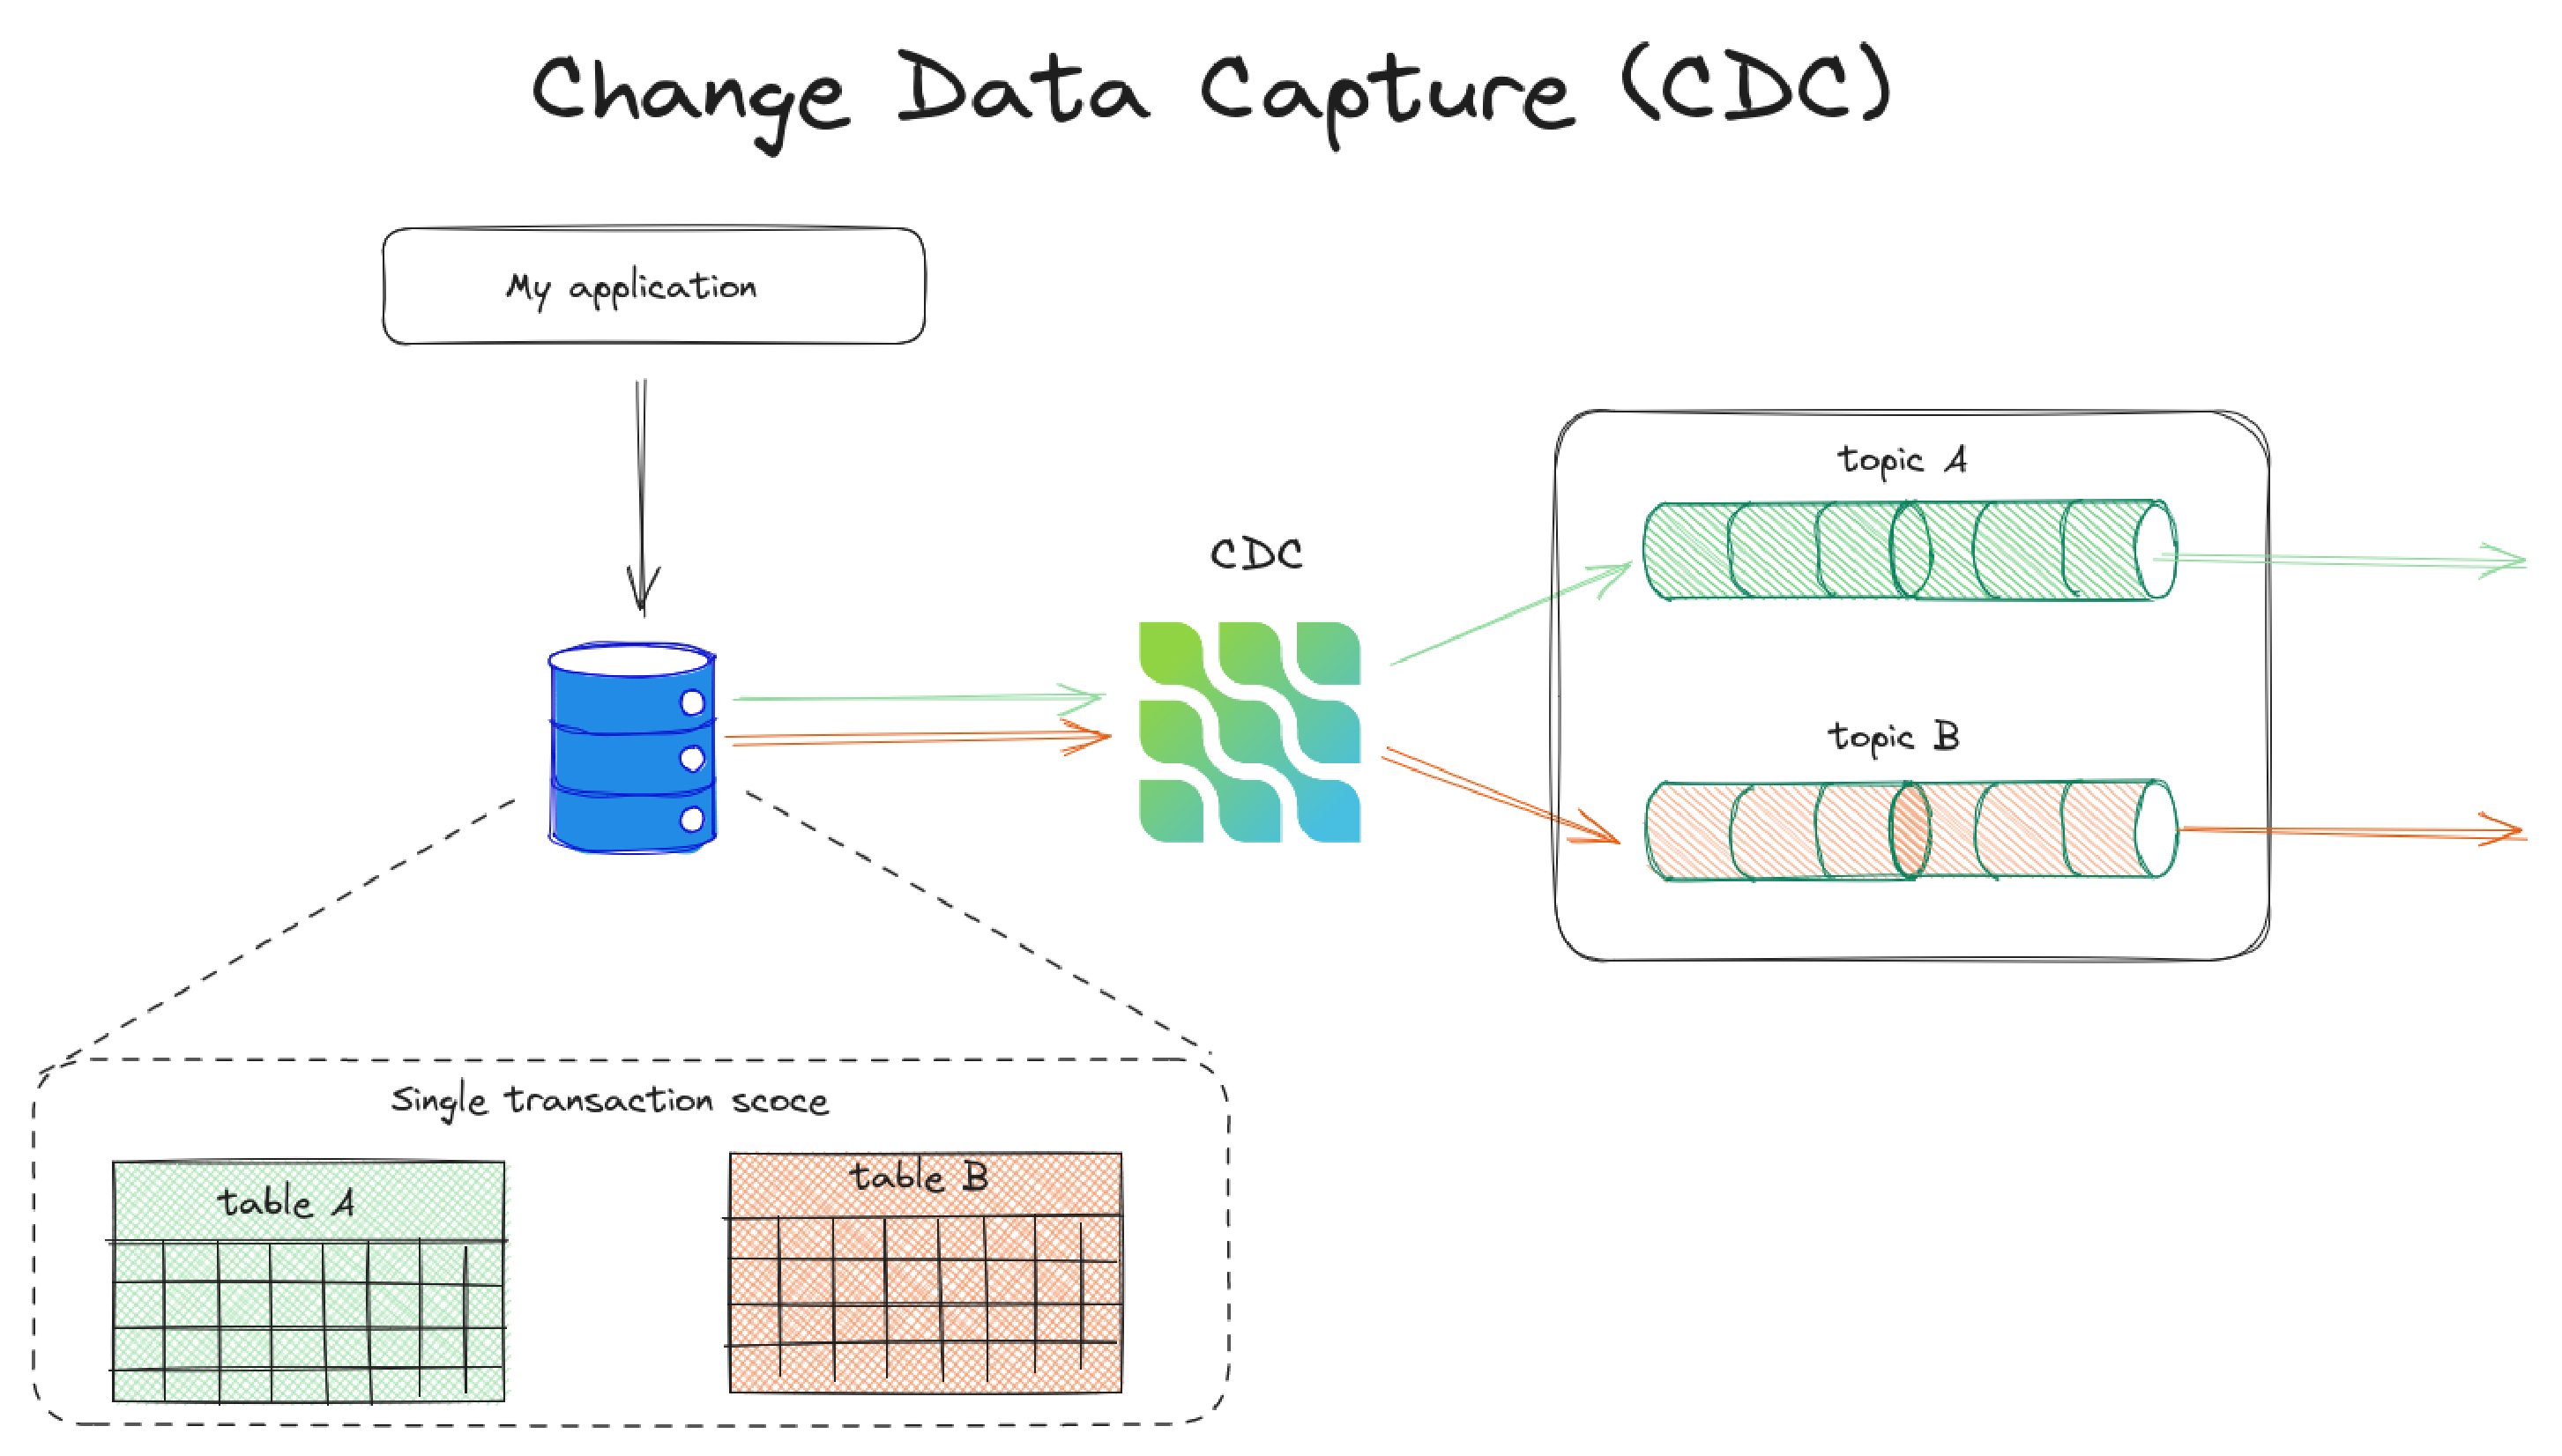
\includegraphics[height=7cm]{./img/cdc.eps}
    \end{figure}
\end{frame}

\begin{frame}
    \begin{figure}
        \centering
        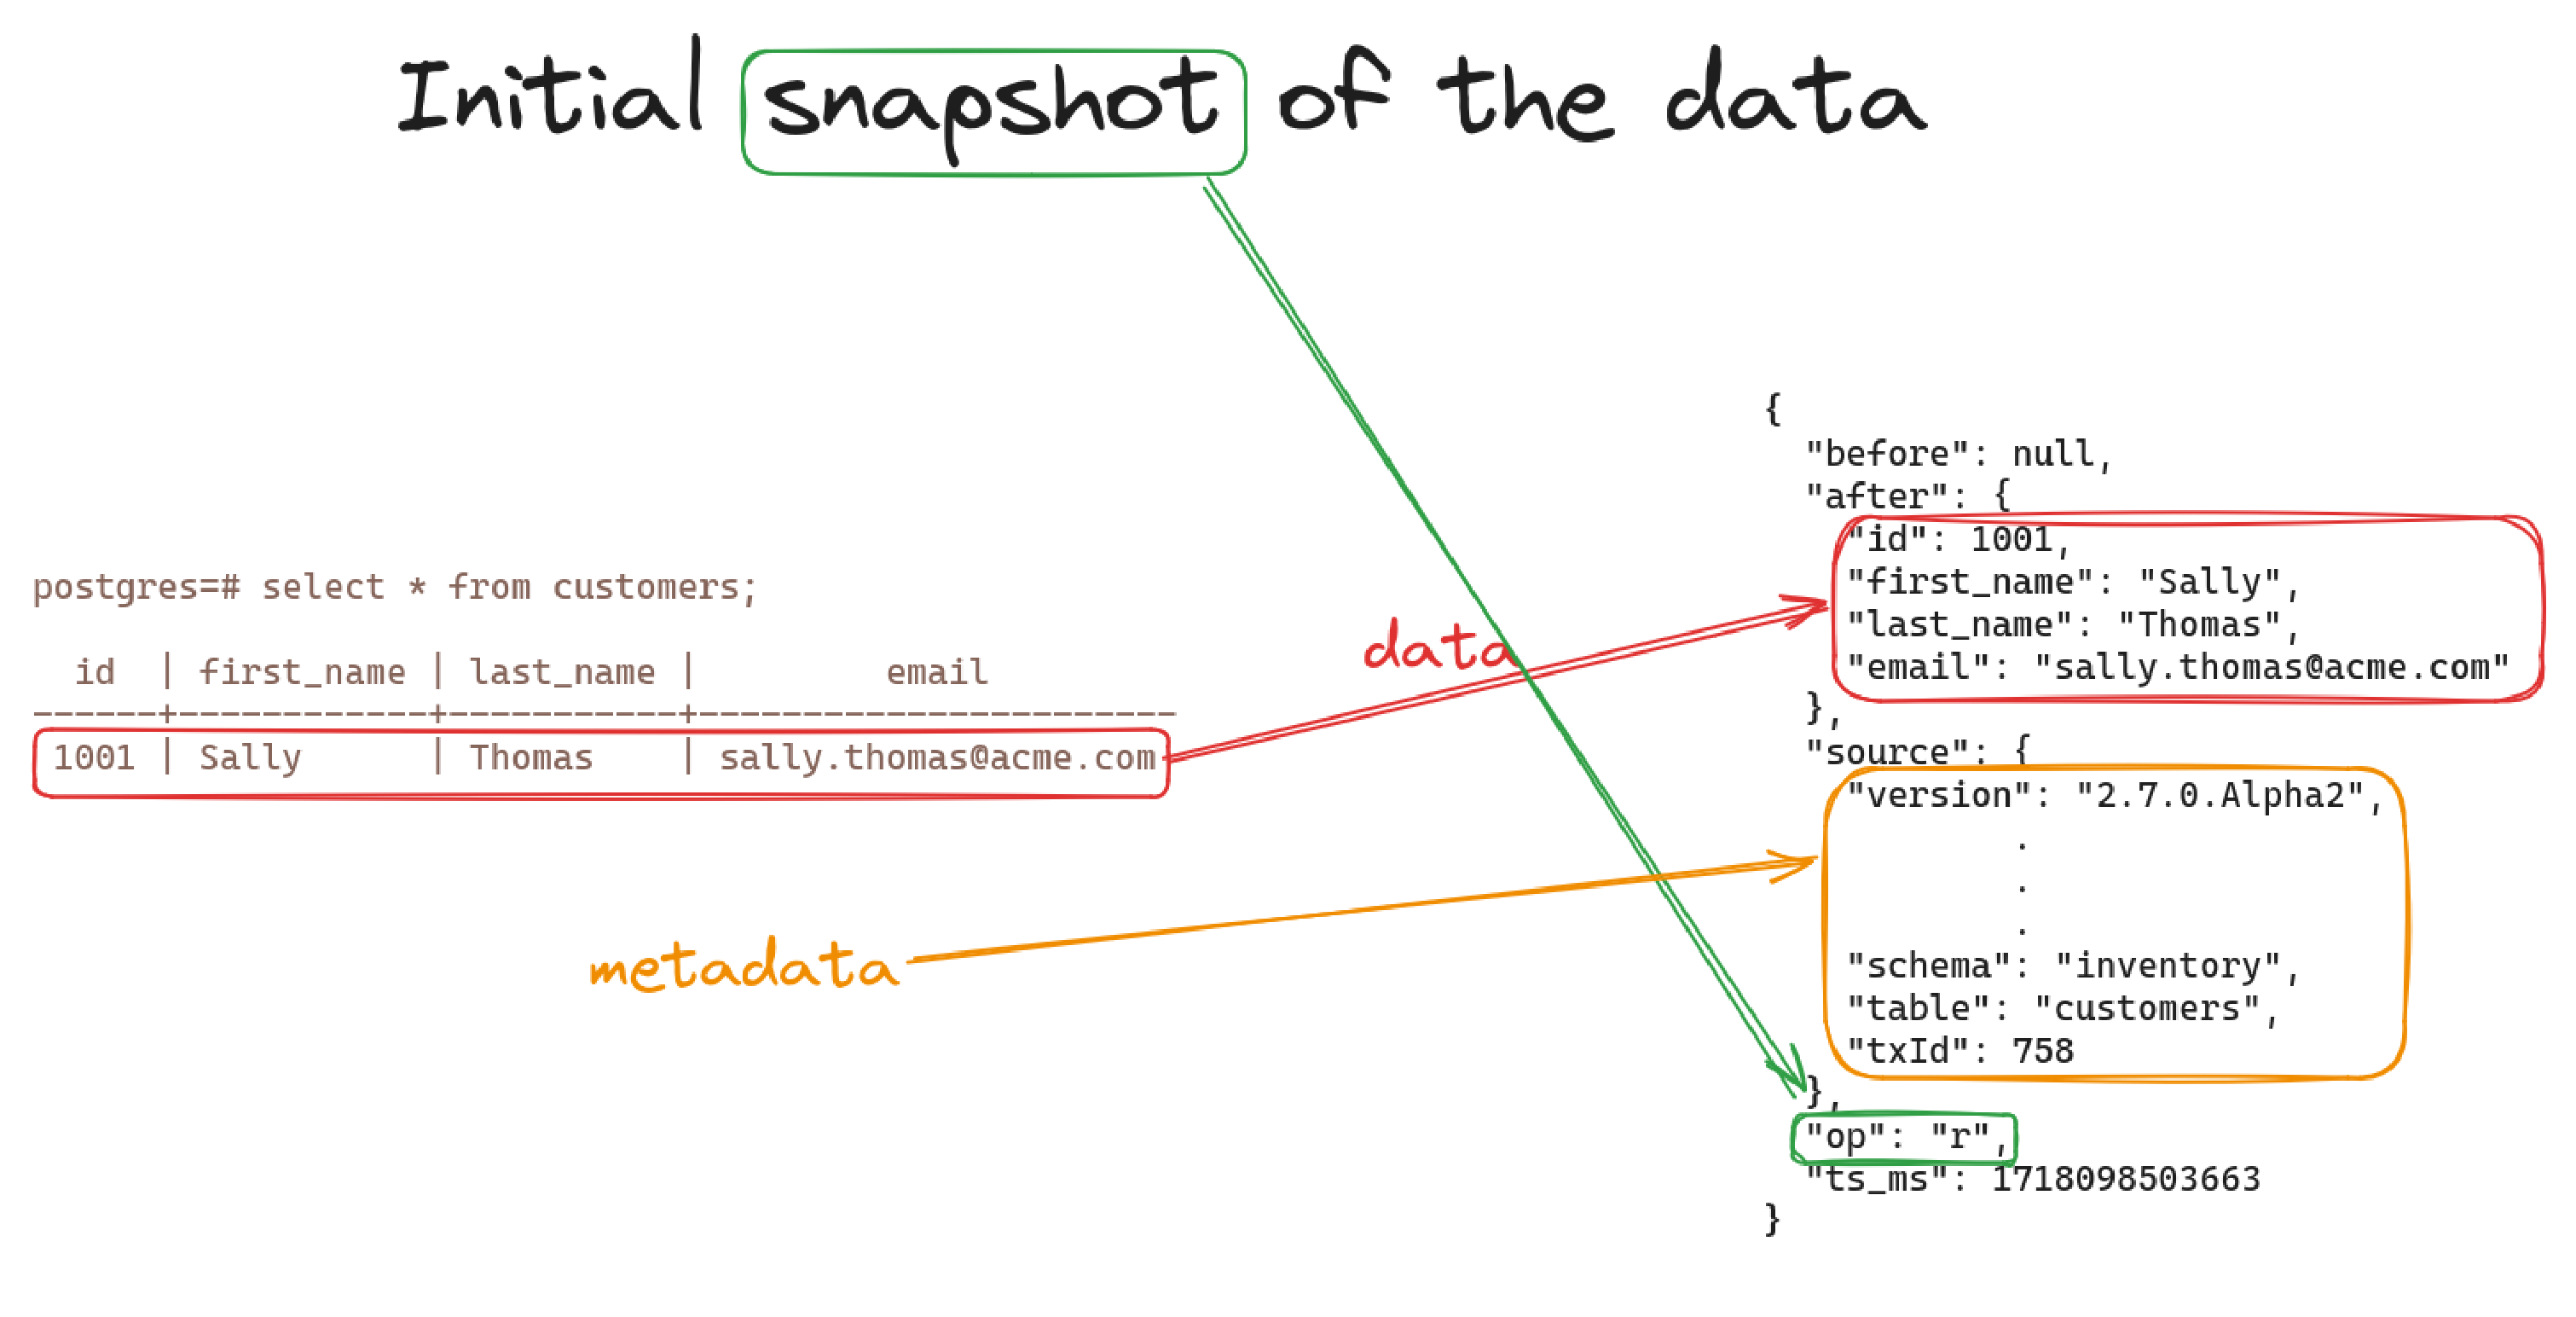
\includegraphics[height=6cm]{./img/initial_snapshot_data.eps}
    \end{figure}
\end{frame}

\begin{frame}
    \begin{figure}
        \centering
        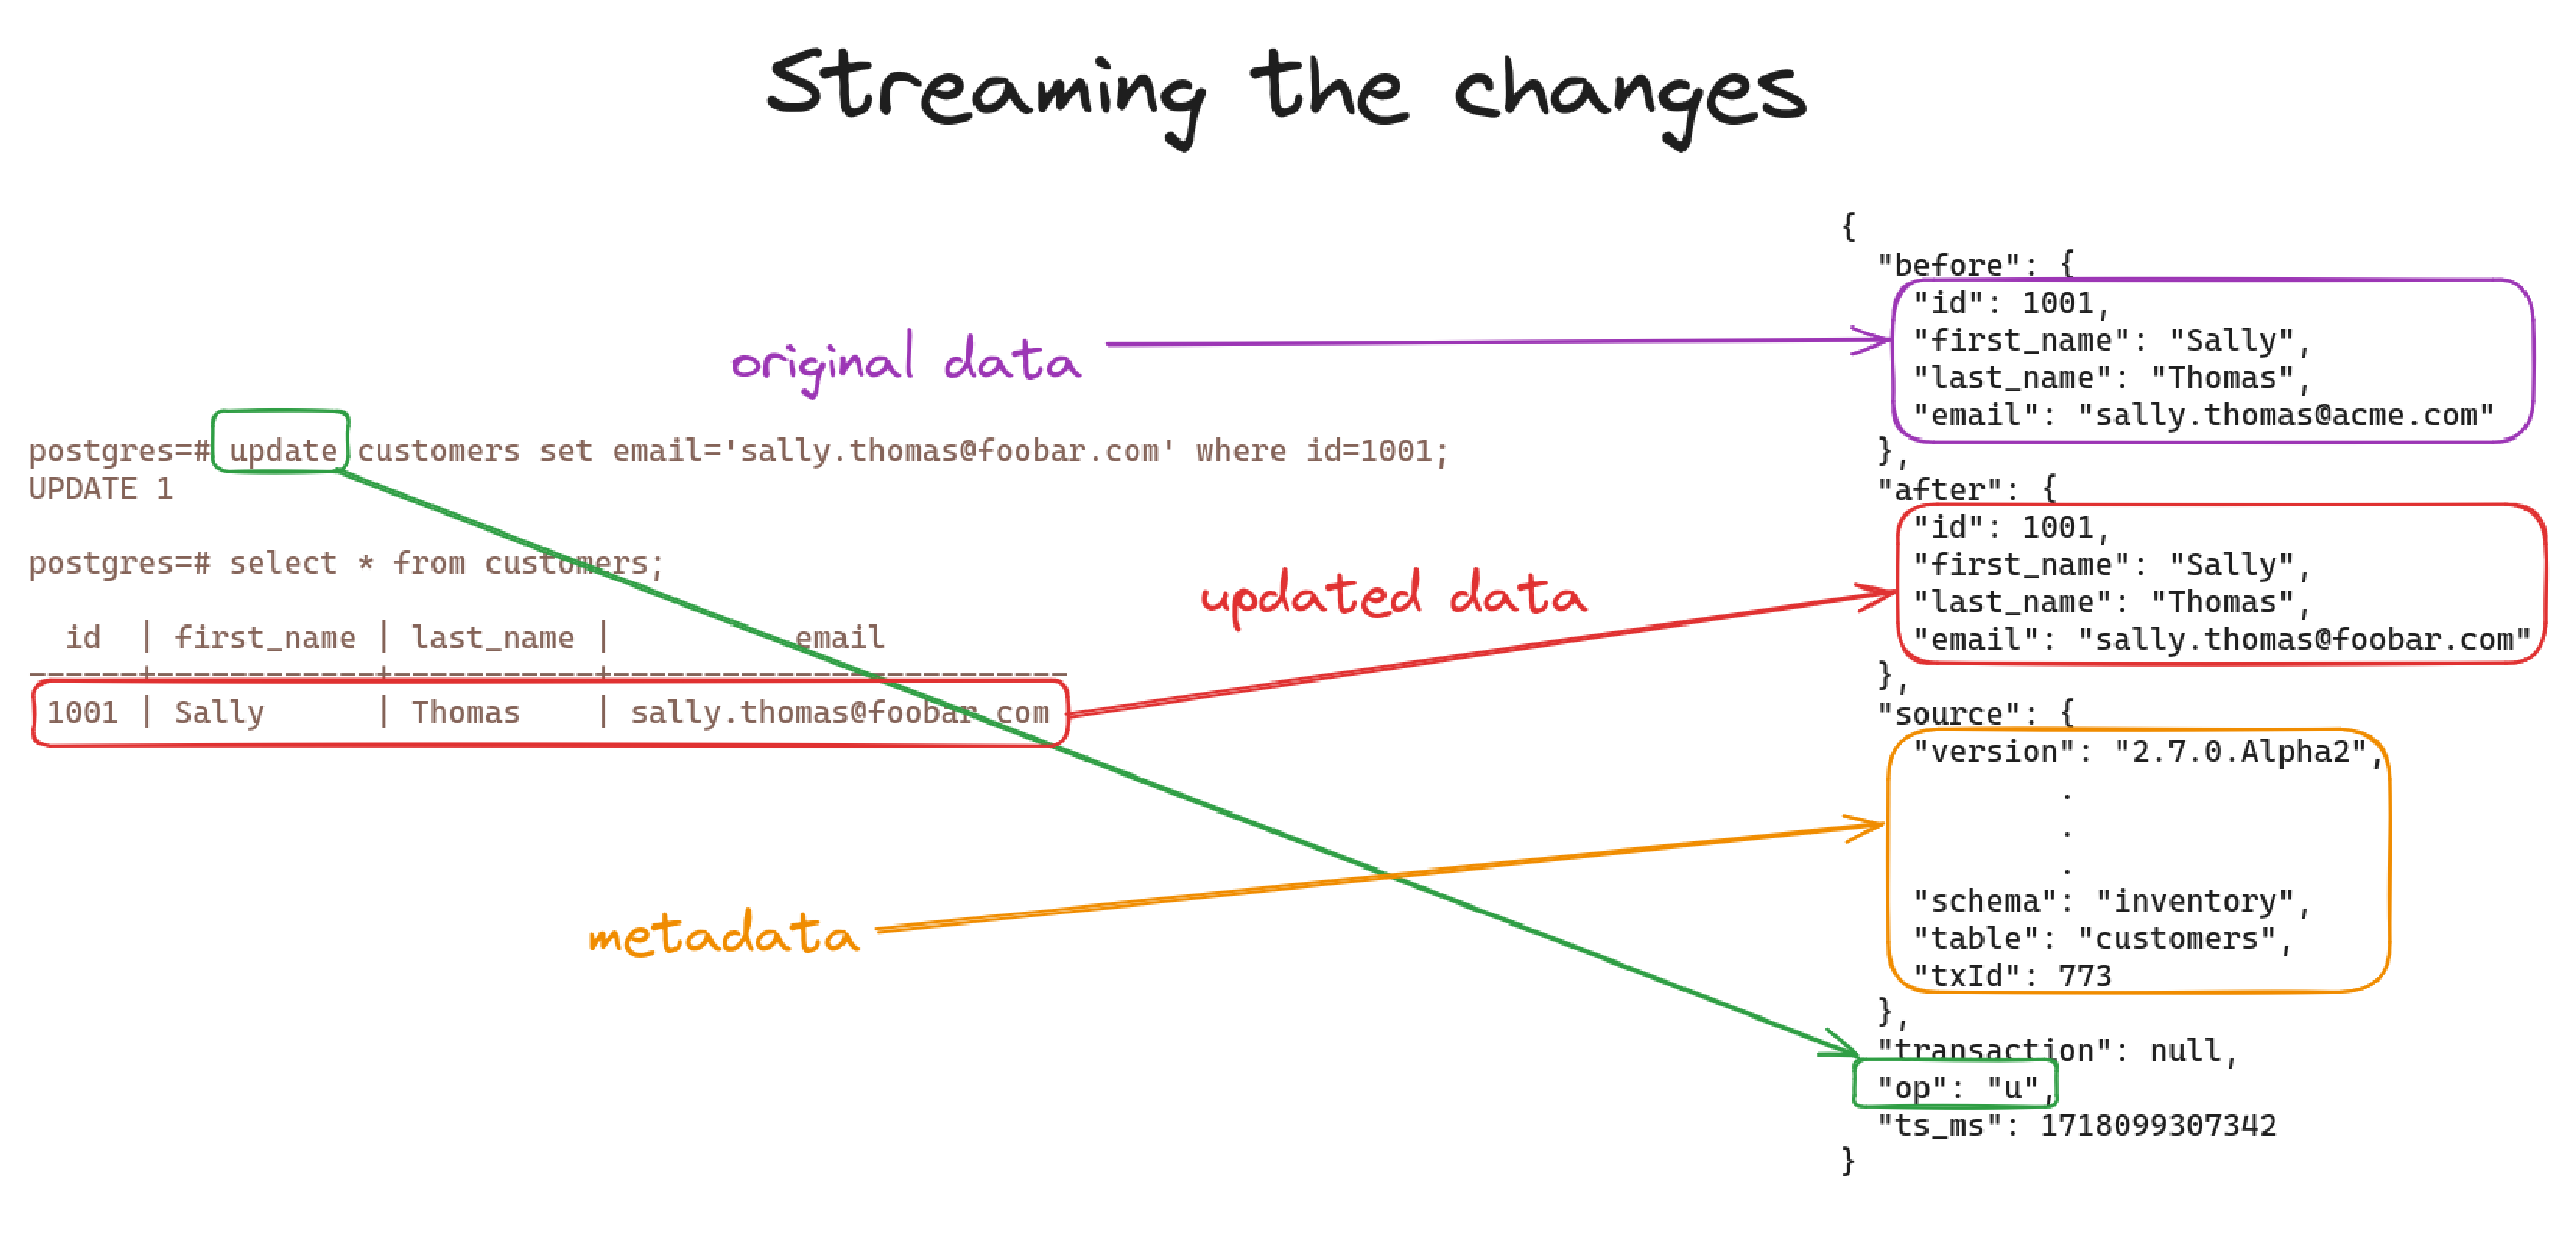
\includegraphics[height=5.5cm]{./img/update_data.eps}
    \end{figure}
\end{frame}

\begin{frame}
    \begin{figure}
        \centering
        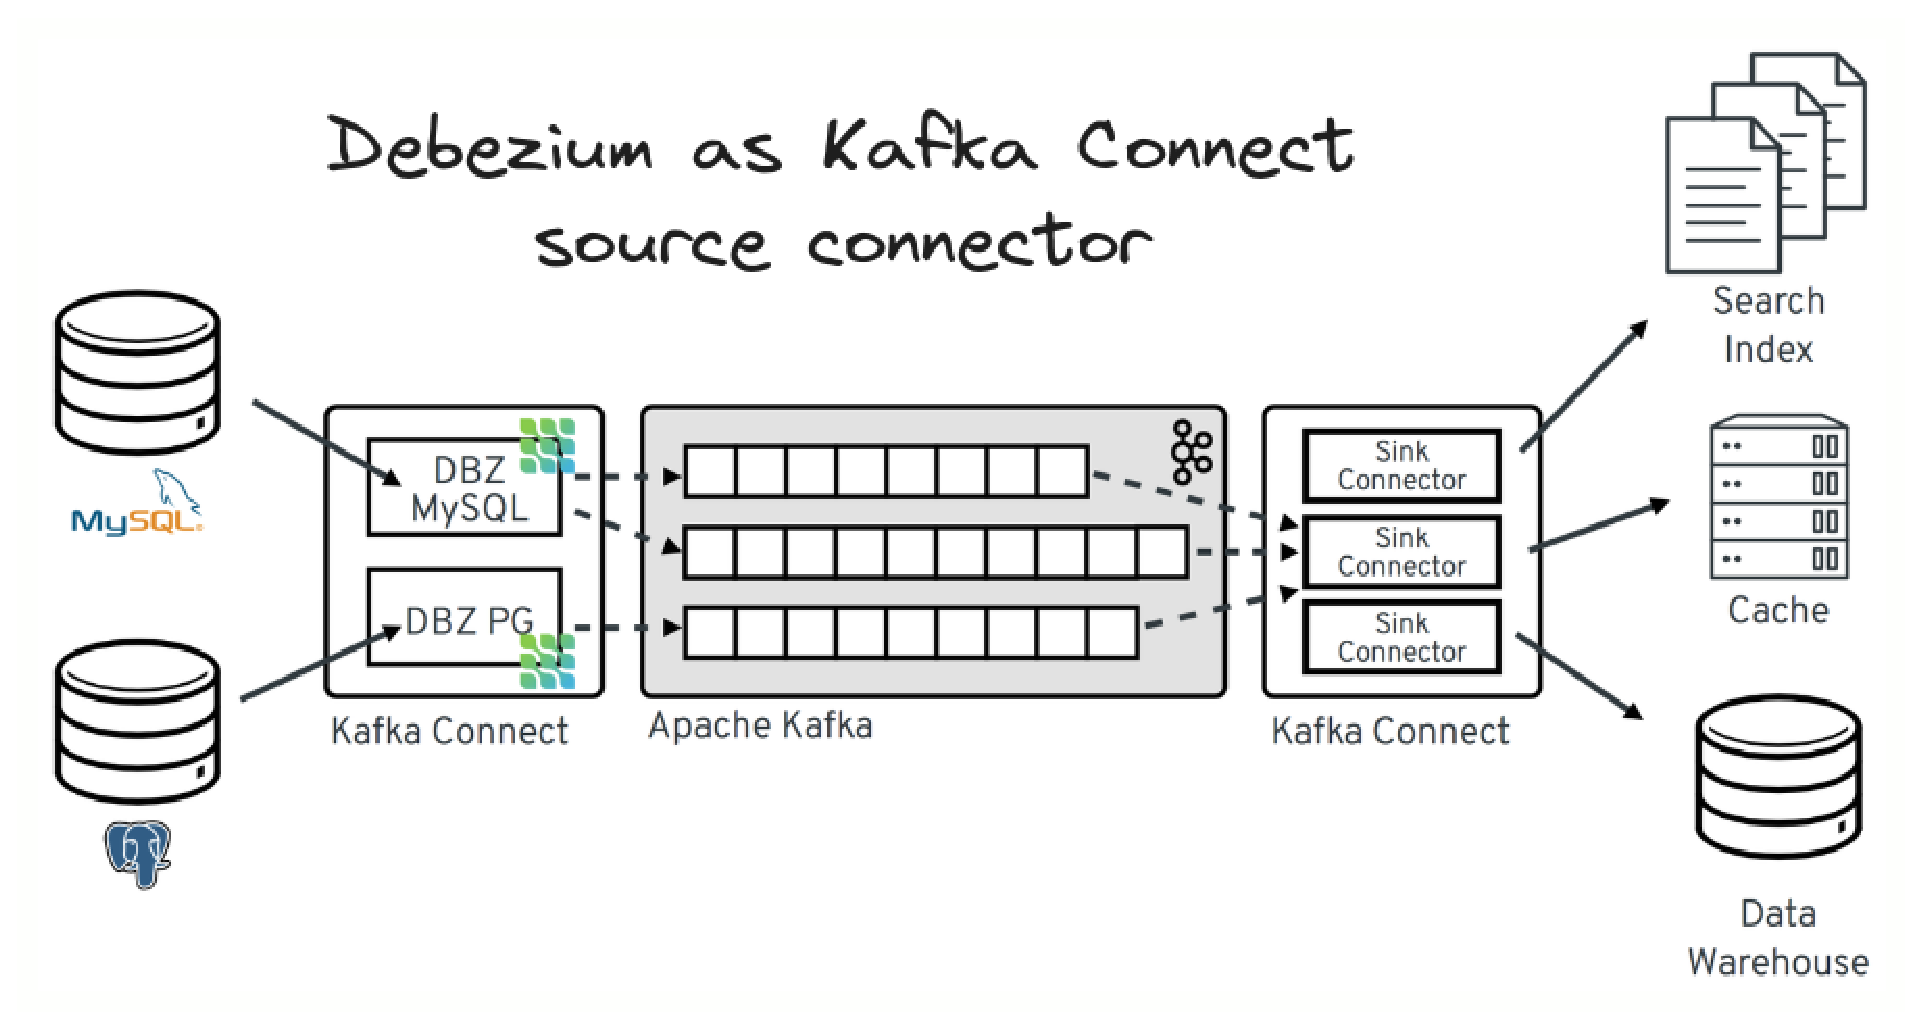
\includegraphics[height=6cm]{./img/debezium_kafka.eps}
    \end{figure}
\end{frame}    
    
\begin{frame}
    \begin{figure}
        \centering
        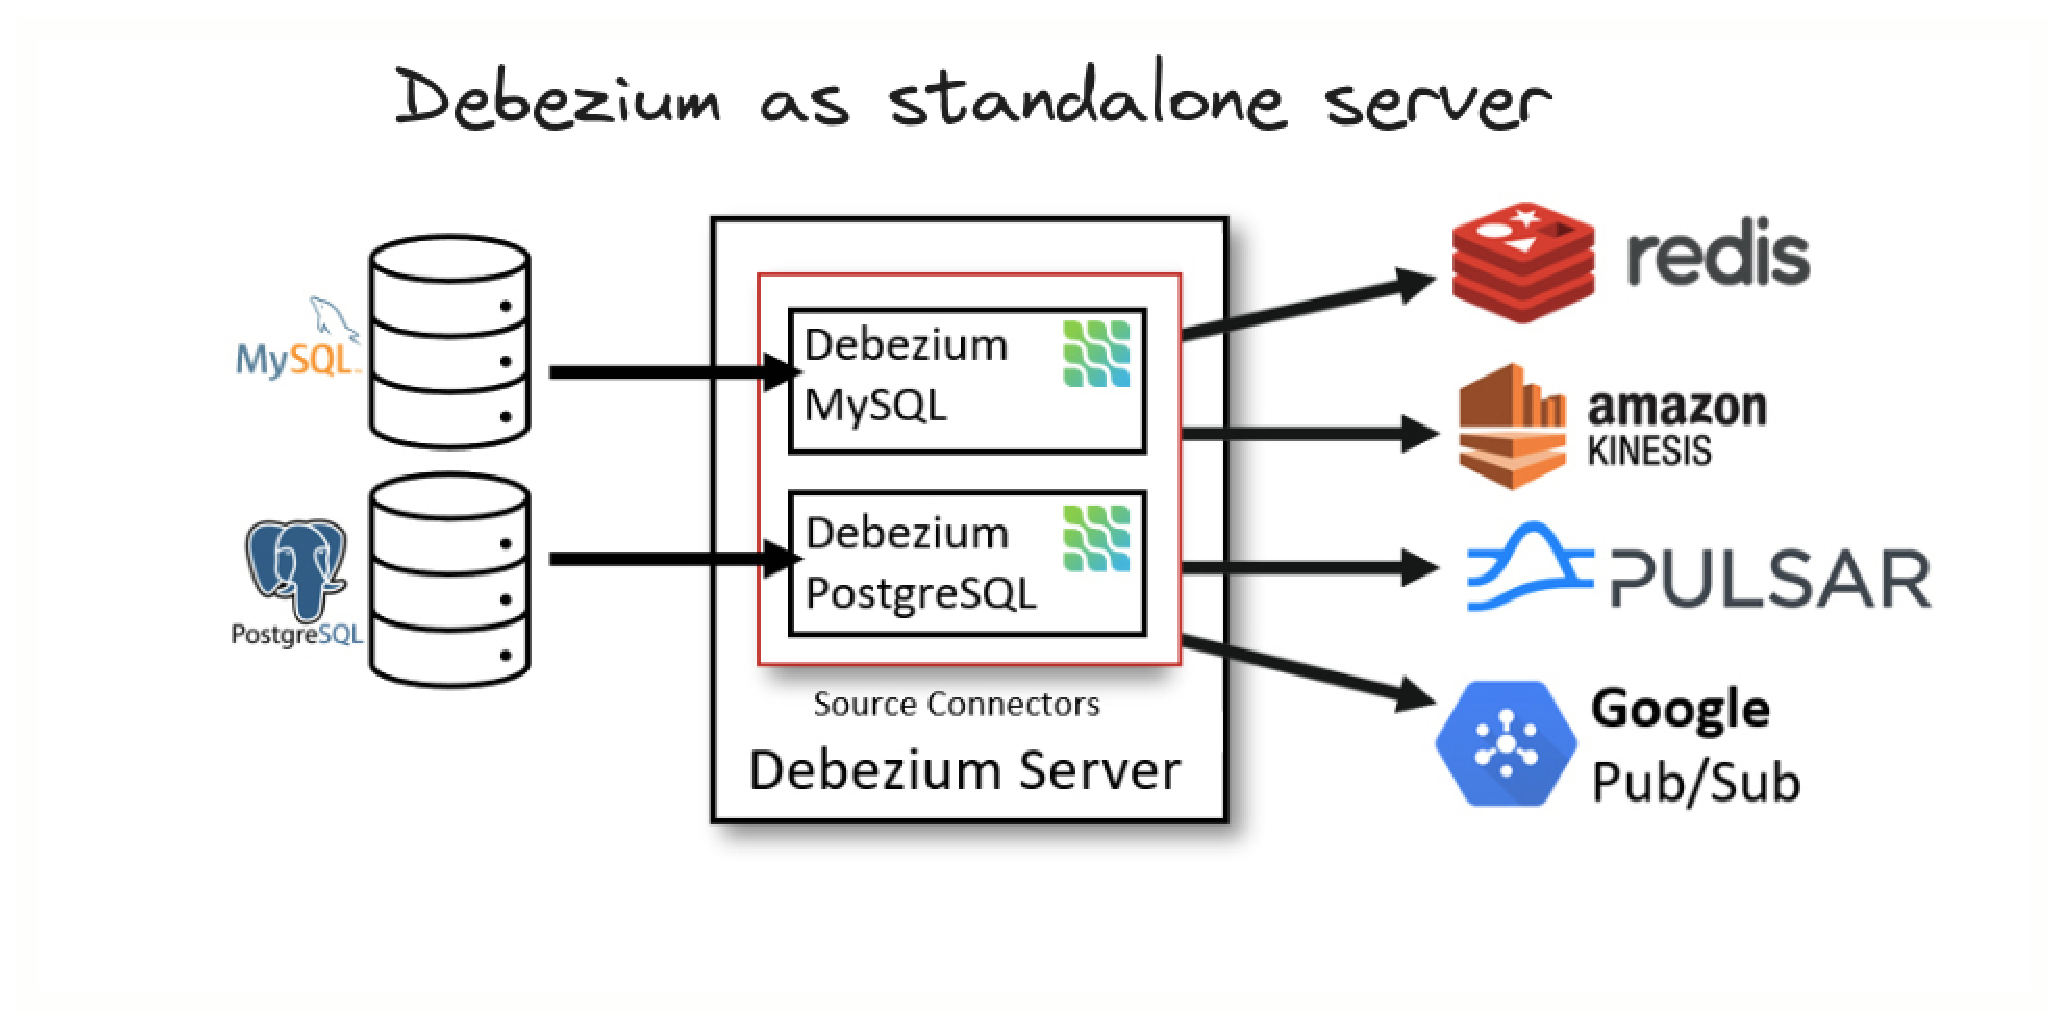
\includegraphics[height=6cm]{./img/debezium_server.eps}
    \end{figure}
\end{frame}    

\begin{frame}
    \begin{figure}
        \centering
        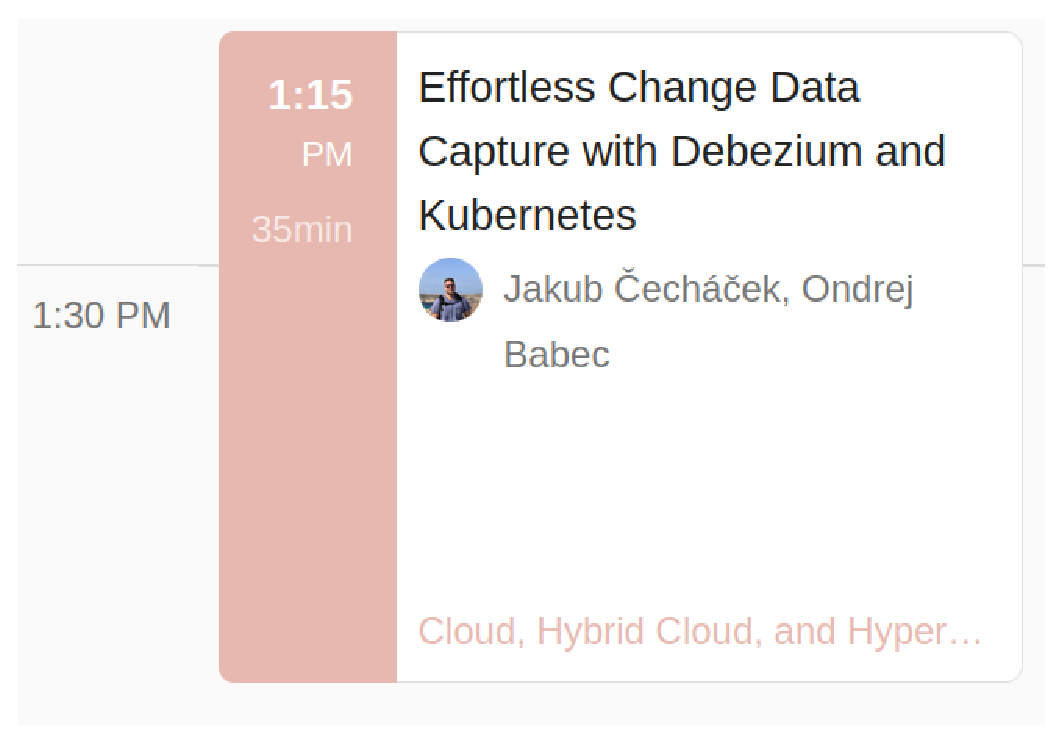
\includegraphics[height=8cm]{./img/dbz_k8s_talk.eps}
    \end{figure}
\end{frame}

\begin{frame}
    % \frametitle{Debezium}
    \vspace*{-1cm}
    \begin{figure}
        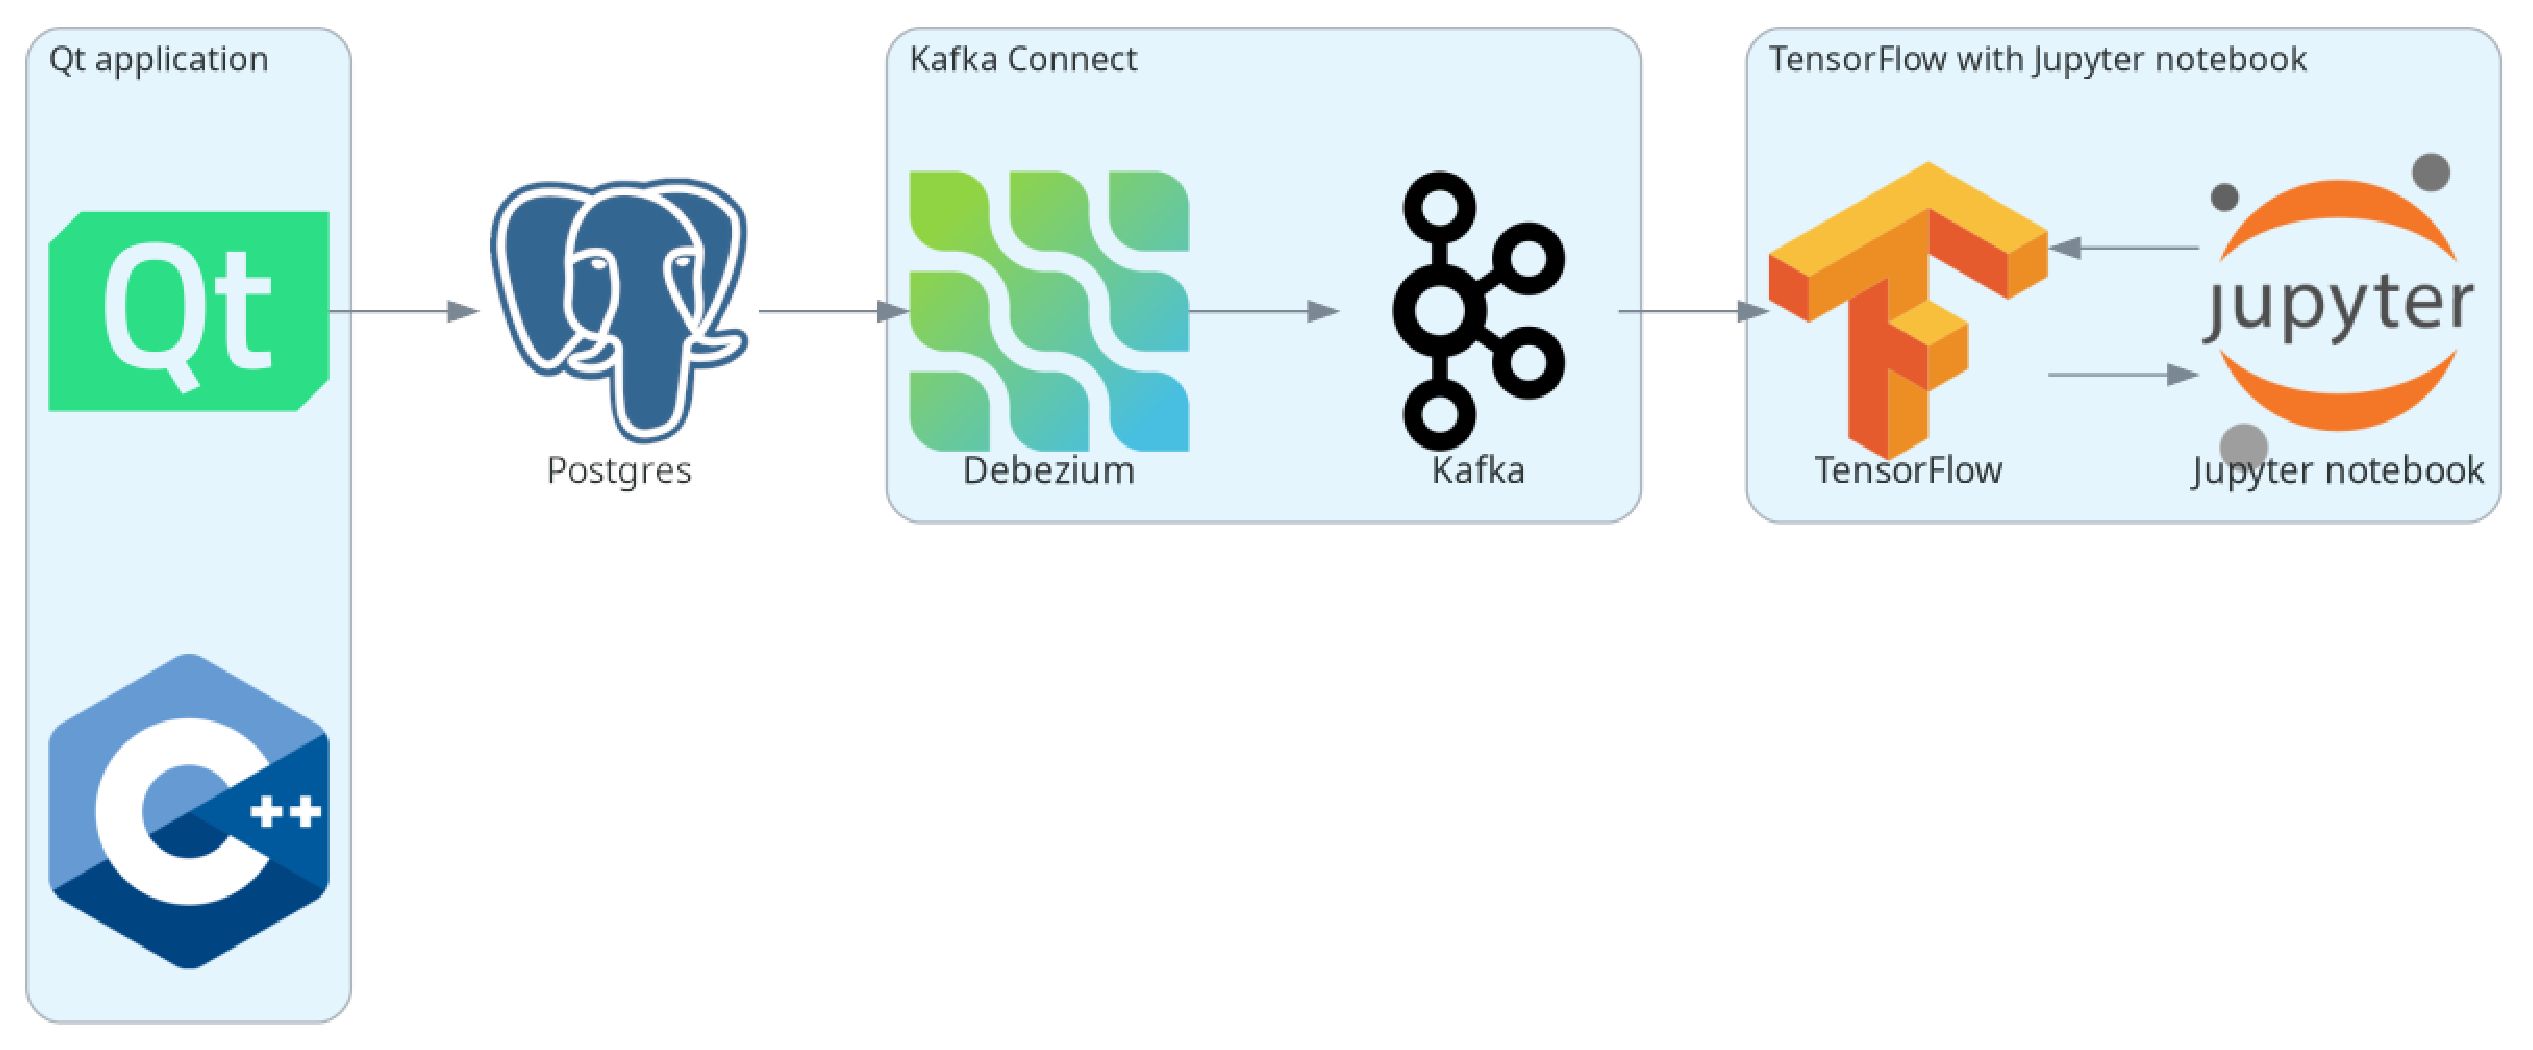
\includegraphics[height=5cm]{./img/qt_to_tf.eps}
    \end{figure}
    
    For more details see
    \begin{itemize}
        \color{blue}
        \item \href{https://debezium.io/blog/2023/05/02/tensorflow-mnist-classification}{Image classification with Debezium and TensorFlow blog post}
        \item \href{https://github.com/debezium/debezium-examples/tree/main/machine-learning/tensorflow-mnist}{Full example on GitHub}
        \color{black}
    \end{itemize}
\end{frame}


\begin{frame}[fragile]
    \frametitle{Debezium configuration}
    \footnotesize
    \begin{lstlisting}[language=json, mathescape=true]
{
  "name": "mnist-connector",
  "config": {
    "connector.class": "io.debezium.connector.postgresql.PostgresConnector",
    "tasks.max": "1",
    "database.hostname": "postgres",
    "database.port": "5432",
    "database.user": "postgres",
    "database.password": "postgres",
    "database.dbname" : "postgres",
    "topic.prefix": "tf",
    $\textcolor{red}{\textbf{"table.include.list": "public.mnist\_.*",}}$
    "key.converter": "org.apache.kafka.connect.storage.StringConverter",
    "value.converter": "org.apache.kafka.connect.storage.StringConverter",
    "transforms": "unwrap, mnist",
    "transforms.unwrap.type": "io.debezium.transforms.ExtractNewRecordState",
    "transforms.mnist.type": "io.debezium.transforms.MnistToCsv"
  }
} 
     \end{lstlisting}
\end{frame}

\begin{frame}[fragile]
    \frametitle{Reading data in TensorFlow}
    \vspace{-0.2cm}
    \footnotesize
    \begin{python}
# define function for decoding Kafka records
def decode_kafka_stream_record(message, key):
    img_int = tf.io.decode_csv(message, [[0.0] for i in range(NUM_COLUMNS)])
    img_norm = tf.cast(img_int, tf.float32) / 255.
    label_int = tf.strings.to_number(key, out_type=tf.dtypes.int32)
    return (img_norm, label_int)
# define Kafka data stream
test_ds = tfio.experimental.streaming.KafkaGroupIODataset(
    topics=[KAFKA_TEST_TOPIC],
    group_id=KAFKA_CONSUMER_GROUP,
    servers=KAFKA_SERVERS,
    stream_timeout=KAFKA_STREAM_TIMEOUT,
    configuration=[
        "session.timeout.ms=10000",
        "max.poll.interval.ms=10000",
        "auto.offset.reset=earliest"
    ],
)
# read batches of Kafka records
test_ds = test_ds.map(decode_kafka_stream_record)
test_ds = test_ds.batch(BATCH_SIZE)
# make predictions on the data samples
model.evaluate(test_ds)
    \end{python}
\end{frame}

\begin{frame}
    \begin{figure}
        \hspace*{-1.1cm}
        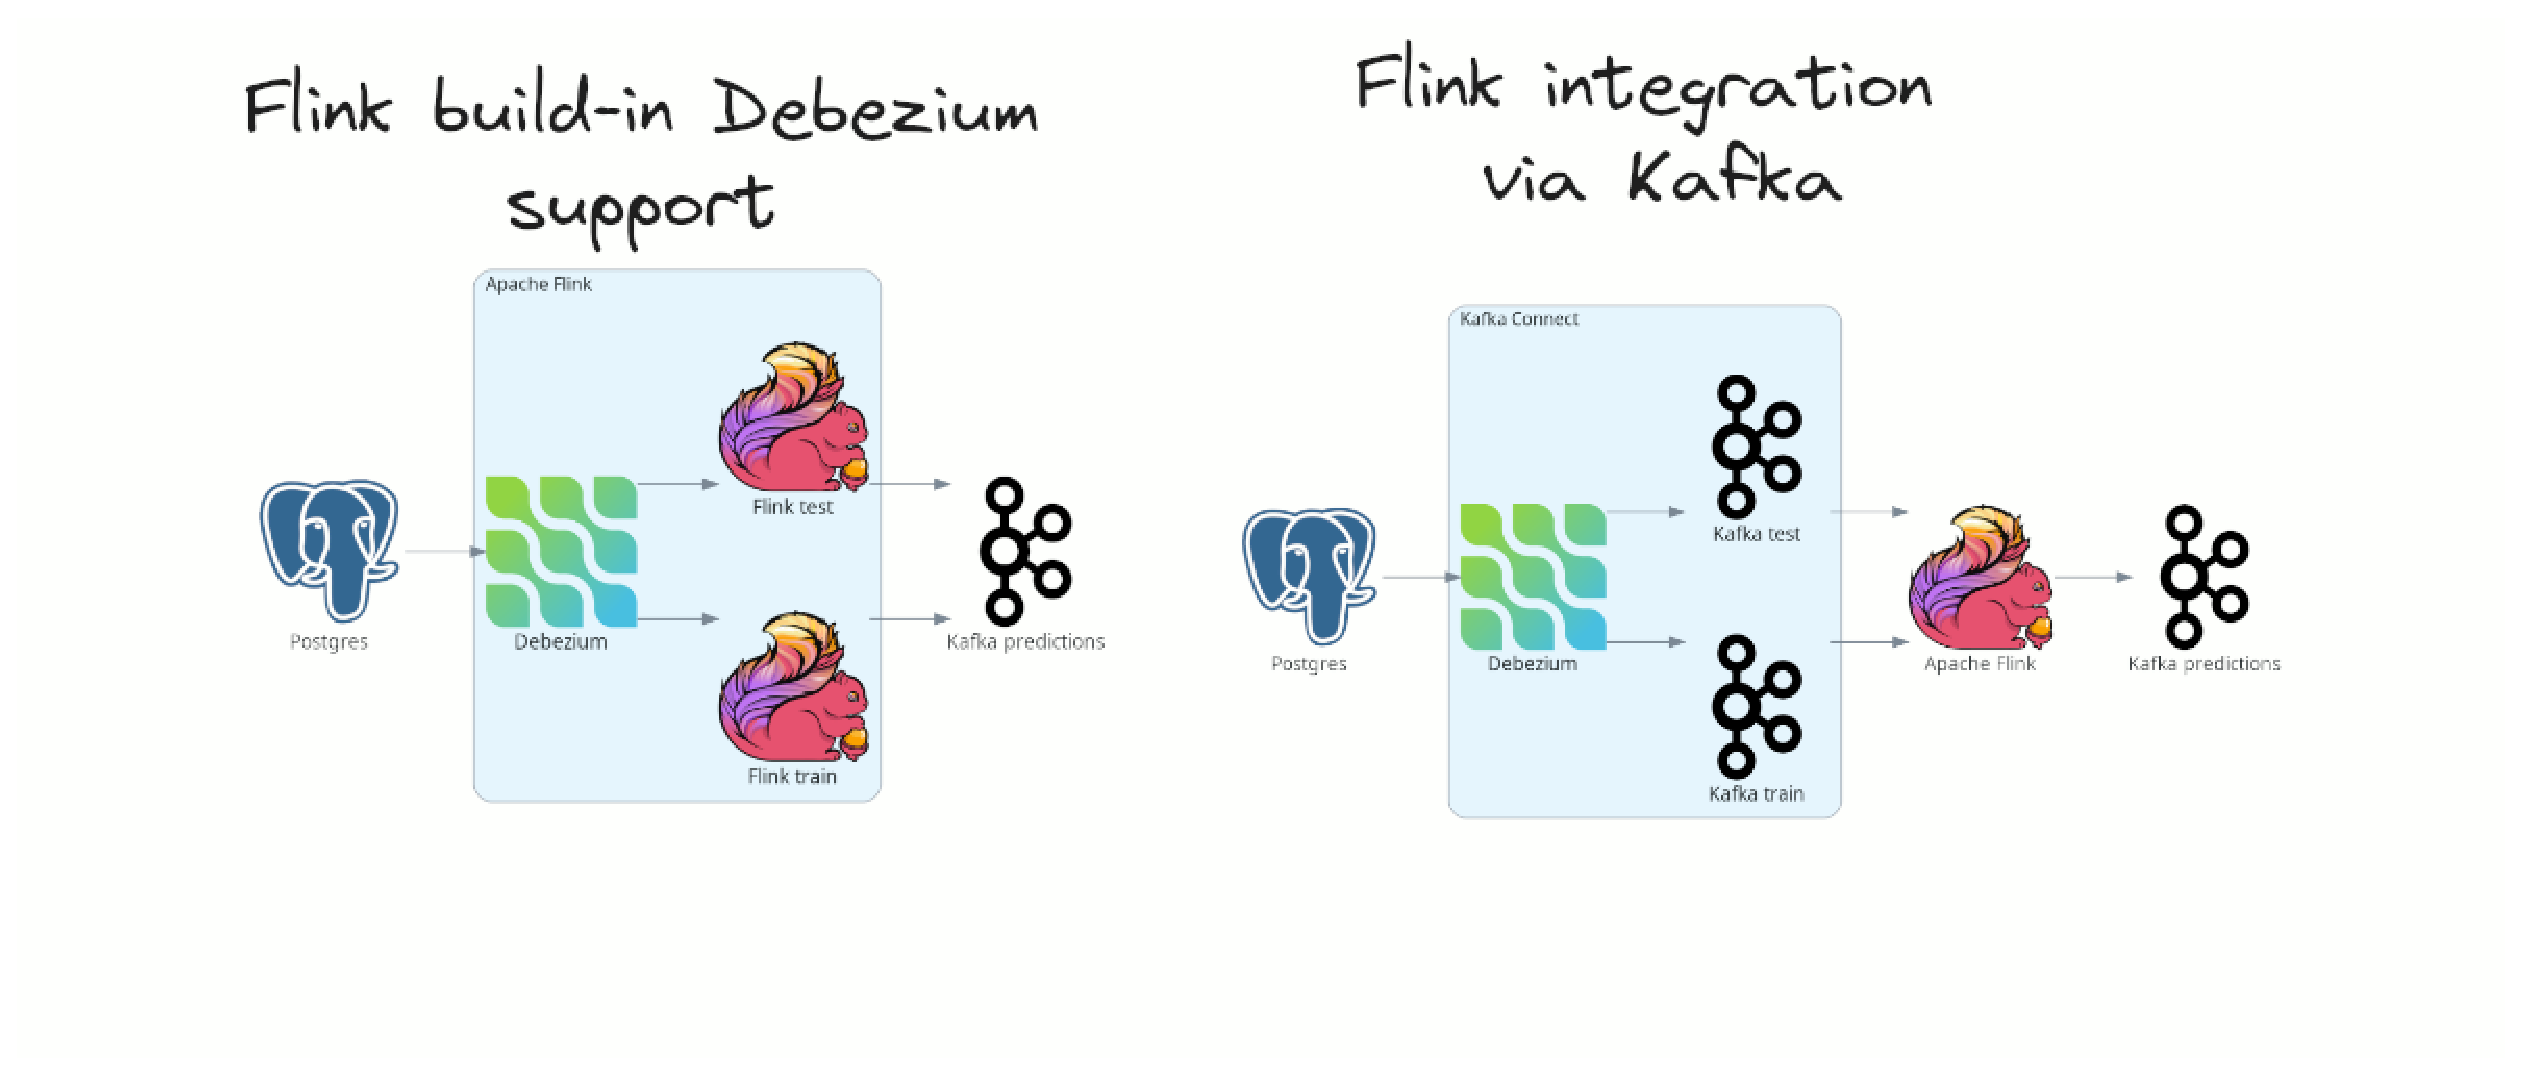
\includegraphics[height=6cm]{./img/debezium_flink.eps}
    \end{figure}
    
    \vspace{-1cm}
    Similar for Apache Spark.
    \vspace{0.5cm}
    
    For more details see
    \begin{itemize}
        \item  \footnotesize \color{blue}\url{https://debezium.io/blog/2023/09/23/flink-spark-online-learning}
        \item  \footnotesize \url{https://github.com/debezium/debezium-examples/tree/main/machine-learning/flink-spark-iris}\color{black}
    \end{itemize}
\end{frame}


\begin{frame}
    \begin{figure}
        \centering
        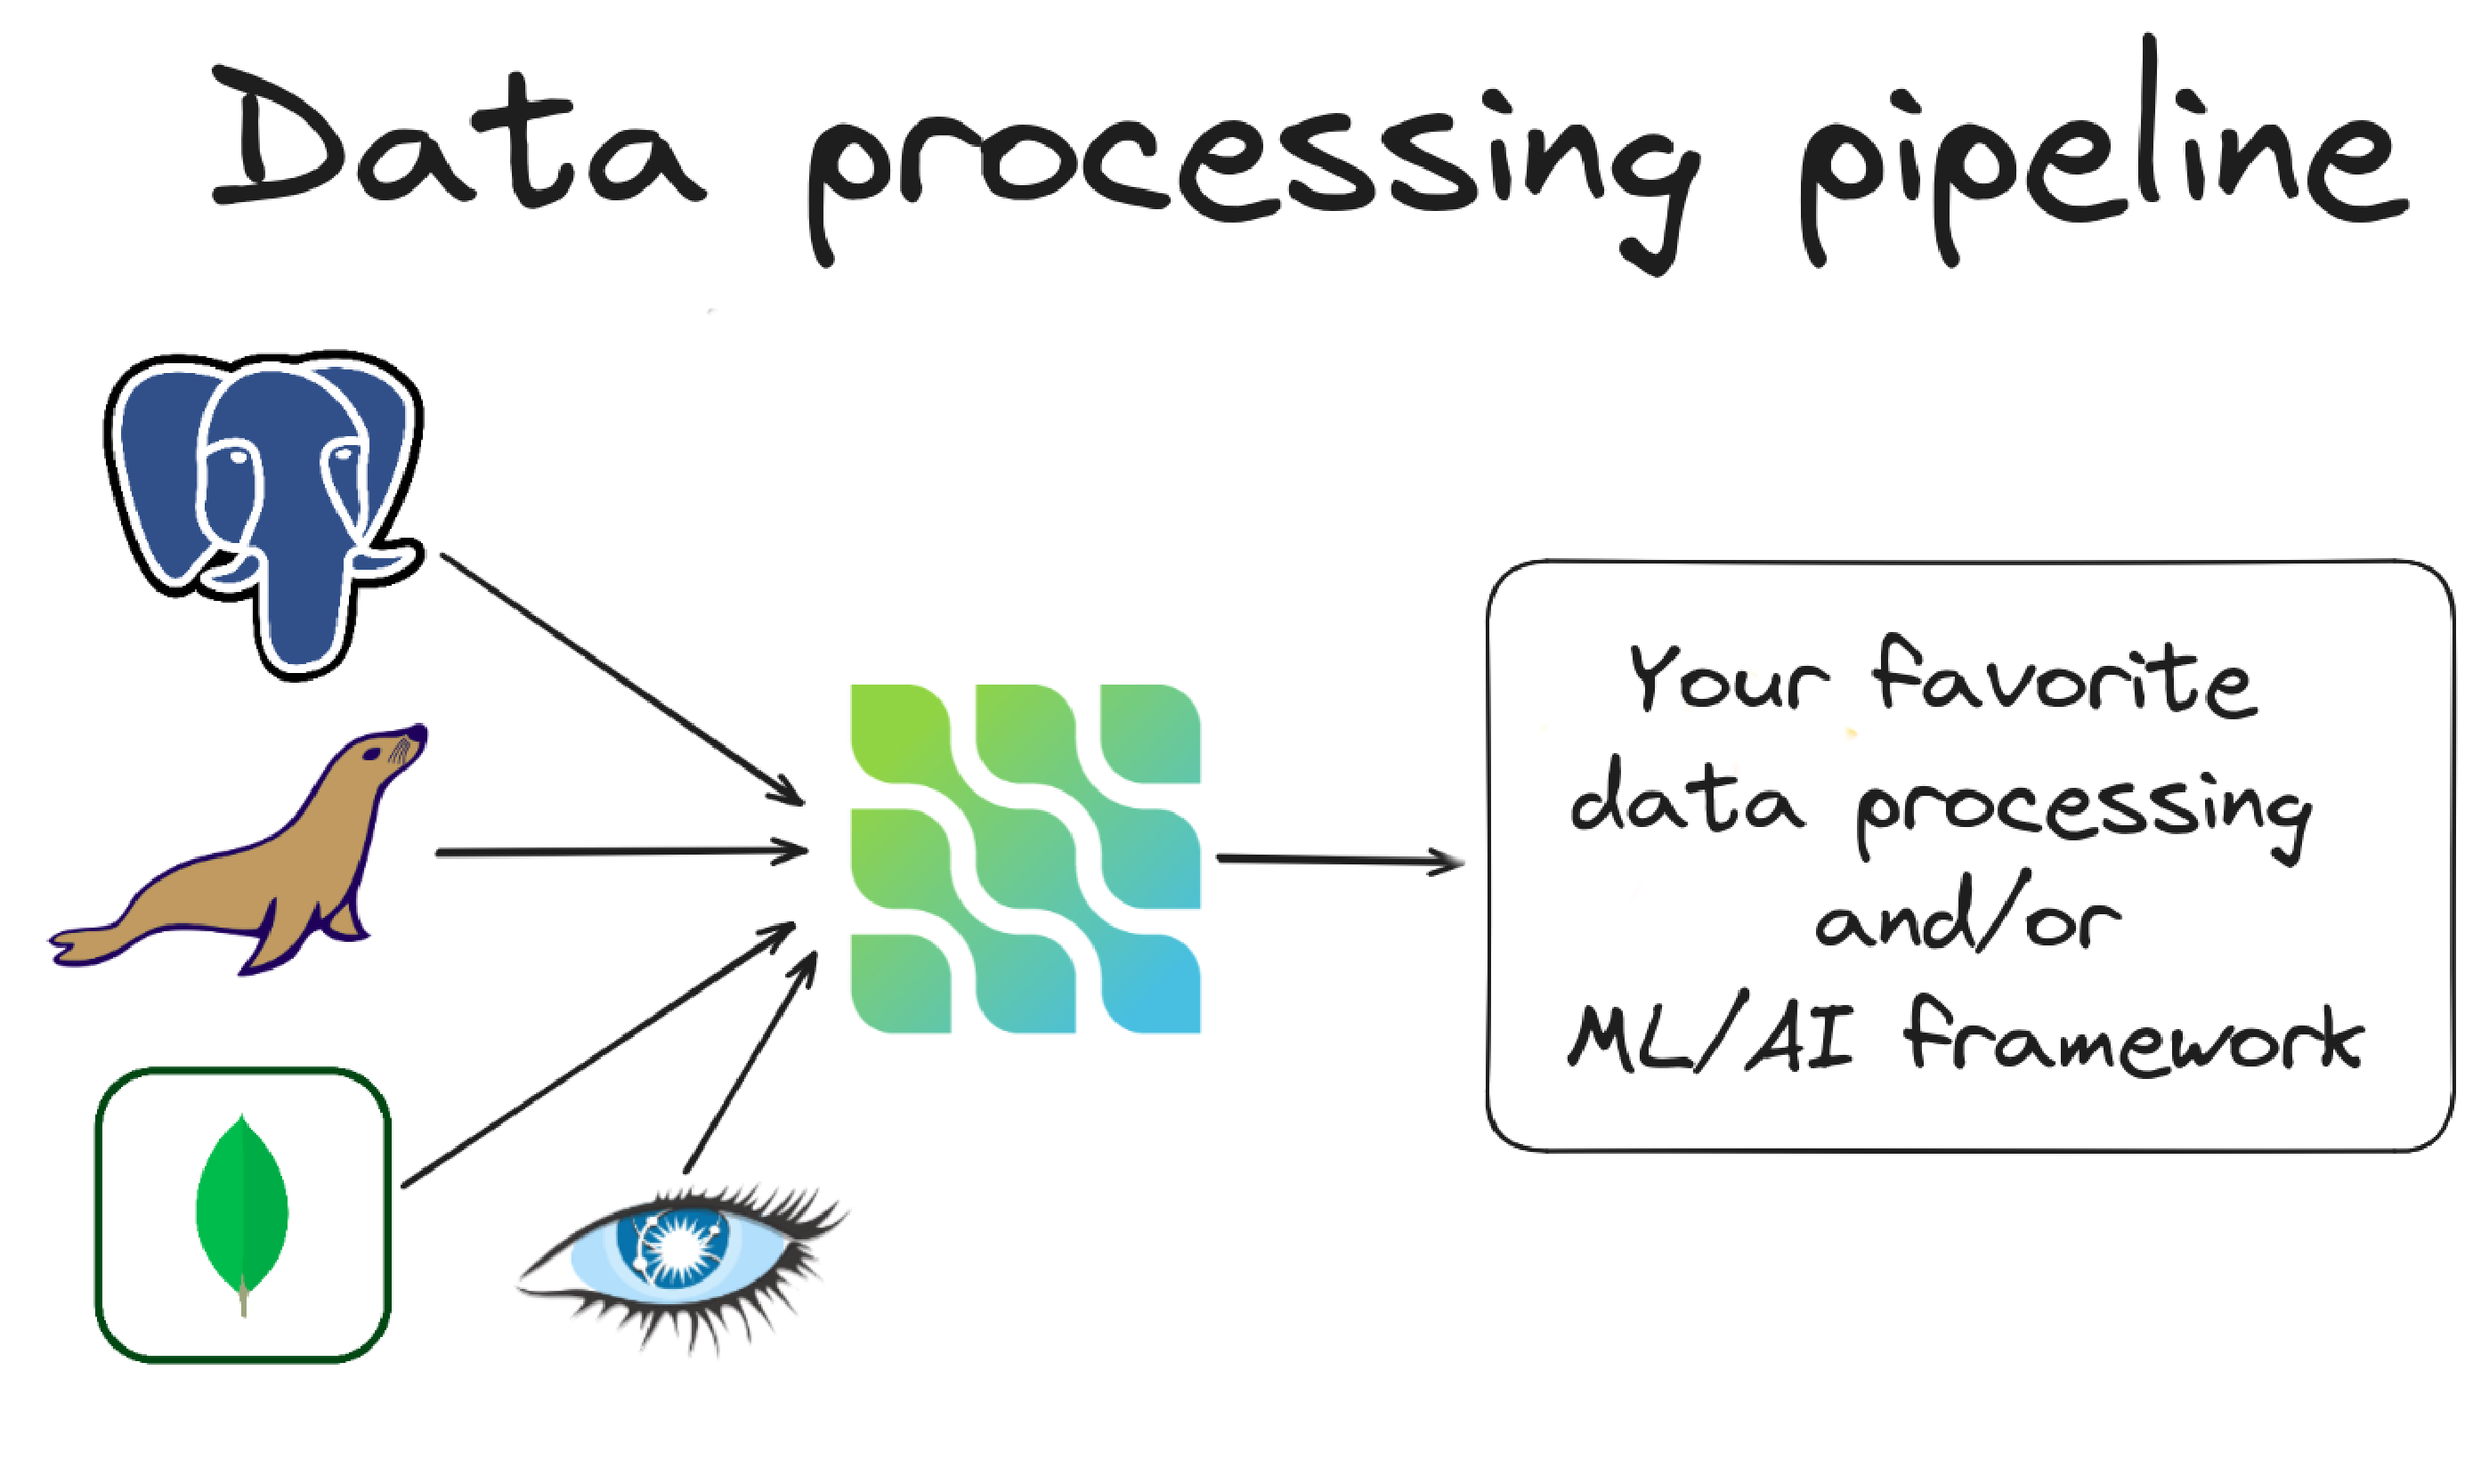
\includegraphics[height=6cm]{./img/dbs_to_ml.eps}
    \end{figure}
\end{frame}

\begin{frame}
    \centering
    \textbf{\Huge{Thank you!}}
    
    \vspace{1cm}
    
    \begin{figure}
        \centering
        
\includegraphics[height=1.5cm]{./img/debezium.eps}
    \end{figure}
    
    \vspace{0.5cm}
    
    \centering
    \color{blue}
    \url{https://debezium.io}\\
    \url{https://github.com/debezium}\\
    \url{https://debezium.zulipchat.com}\\
    \url{https://groups.google.com/g/debezium}\\
    \color{black}
\end{frame}

%%%%%%%%%%%%%%%%%%%%%%%%%%%%%%%%%%%%%%%%%%%%%%%%%%%%%%%%%%%%%%%%%%%%%%%%%%%%%%%%%%%%%%%%%%%%%%%%%
%%% BACKUP
%%%%%%%%%%%%%%%%%%%%%%%%%%%%%%%%%%%%%%%%%%%%%%%%%%%%%%%%%%%%%%%%%%%%%%%%%%%%%%%%%%%%%%%%%%%%%%%%%

% \begin{frame}
%     \centering
%     \huge{\textbf{Backup slides}}
% \end{frame}

\end{document}
